%-*- coding: UTF-8 -*-
\documentclass[UTF8]{ctexart}
\usepackage{graphicx}
\usepackage{float}
\usepackage{amsmath}
\usepackage[a4paper,hmargin=2.5cm,vmargin=2.0cm,includeheadfoot]{geometry}
\usepackage[format=hang,font=bf,sf,normalsize]{caption}
\usepackage[nottoc]{tocbibind}
\usepackage{subfig}

\usepackage[noend]{algpseudocode}%伪代码
\usepackage{algorithmicx,algorithm}
\usepackage{tabularx}%插入表格
\usepackage{booktabs}
\usepackage{multirow}

\usepackage{fontspec}
\setmainfont[Scale=1.0]{Times New Roman}

\usepackage{titlesec} %改变各标题格式
\newfontfamily\sectionef{Arial}	
\titleformat{\section}{\centering \zihao{-2} \heiti \sectionef}{第\,\thesection\,章}{1em}{}
\titleformat*{\subsection}{\raggedright \zihao{3} \heiti \sectionef}
\titleformat*{\subsubsection}{\raggedright \zihao{-3} \heiti \sectionef}

\usepackage{titletoc} %改变目录标题格式
\titlecontents{section}[0cm]{\vspace{12pt} \heiti \zihao{3}}{\hspace*{1em}\contentslabel{2em}\ }%section
{}{\titlerule*[0.5pc]{$\cdot$}\large \contentspage \hspace{0.5cm}}
\titlecontents{subsection}[0.5cm]{\vspace{12pt} \zihao{4} \songti}{\hspace*{2em}\contentslabel{2em}\ }%subsection
{}{\titlerule*[0.5pc]{$\cdot$}\large \contentspage \hspace{0.5cm}}
\titlecontents{subsubsection}[1.0cm]{\vspace{12pt} \zihao{-4} \songti}{\hspace*{2em}\contentslabel{2em}\ }%subsubsection
{}{\titlerule*[0.5pc]{$\cdot$}\large \contentspage \hspace{0.5cm}}

\usepackage{fancyhdr}
\pagestyle{fancy}                   % 设置页眉页脚
\lhead{\heiti GPU并行计算}                   %页眉左侧显示页数                 
\rhead{\heiti \leftmark}                         %章节信息                       
\cfoot{\thepage}                                %当前页           
\renewcommand{\headrulewidth}{0.1pt}
\renewcommand{\footrulewidth}{0.1pt}

\usepackage{zhnumber} % change section number to chinese
\renewcommand\thesection{\zhnum{section}}
\renewcommand\thesubsection{\arabic{section}.\arabic{subsection}}

\usepackage[sort]{natbib} 

\begin{document}
    
    \begin{titlepage}

\newcommand{\HRule}{\rule{\linewidth}{0.5mm}} % Defines a new command for the horizontal lines, change thickness here

%----------------------------------------------------------------------------------------
%	LOGO SECTION
%----------------------------------------------------------------------------------------


\includegraphics[width = 4cm]{./figures/ustcblue}\\[0.5cm] 

\begin{center} % Center remainder of the page

%----------------------------------------------------------------------------------------
%	HEADING SECTIONS
%----------------------------------------------------------------------------------------
\textbf{\Huge GPU并行计算大作业}\\[1.5cm] 
\textup{\huge 中国科学技术大学}\\[0.5cm] 
\textup{\Large }\\[0.5cm] 
%----------------------------------------------------------------------------------------
%	TITLE SECTION
%----------------------------------------------------------------------------------------
\HRule \\[0.4cm]
{ \Huge \bfseries 格子玻尔兹曼方法求解圆柱绕流问题}\\ % Title of your document
\HRule \\[1.5cm]

\end{center}
%----------------------------------------------------------------------------------------
%	AUTHOR SECTION
%----------------------------------------------------------------------------------------
\begin{center} \Large
    \begin{tabular}{cc}
        \makebox[6em][s]{\heiti 姓\hspace{\fill}名:} & 汪乘雲          \\
        \makebox[6em][s]{\heiti 学\hspace{\fill}号:} & SA21005050      \\
        \makebox[6em][s]{\heiti 学\hspace{\fill}院:} & 工程科学学院      \\
        \makebox[6em][s]{\heiti 专\hspace{\fill}业:} & 流体力学     \\
        \makebox[6em][s]{\heiti 授课老师:} & 谭立湘         \\
        \makebox[6em][s]{\heiti 日\hspace{\fill}期:} & \number\year 年 \number\month 月 \number\day 日
    \end{tabular}
\end{center}
\vspace{2cm}
\makeatletter


\vfill % Fill the rest of the page with whitespace

\makeatother

\end{titlepage}


    
    \newpage
    
    \tableofcontents
    \setcounter{page}{0}

    \newpage
    \section{绪论}
        \zihao{-4}
        随着计算机技术的发展和现代流体力学计算方法的不断改进,计算流体力学(CFD)已经成为研究流体力学各种物理现象的重要工具。
        其中主流的算法包括有限体积法,有限差分法以及有限元法等等。

        格子波尔茨曼方法(Lattice Boltzmann Method, LBM)作为诞生只有30多年的新兴算法,其应用一直是CFD领域研究的热点问题之一,
        其理论和应用研究也都取得了长足的进步。作为一种使用微观模型来模拟流体的宏观行为的介观方法,格子玻尔兹曼方法相比于传统的数值方法,
        可以比较方便的处理复杂的边界条件,计算效率更高效且具有很好的并行性,能够在大规模并行计算机上计算。
        由于是基于统计热物理的理论基础,所以在某些传统方法无法胜任的领域,
        比如微尺度流动与换热、多孔介质、磁流体、生物流体等领域,都可以进行有效模拟。

        而随着科技技术的发展,计算流体力学针对的问题也越来越复杂,计算能力的需求也急剧增长,CPU的发展速度已经难以满足。
        目前,GPU 凭借其强大的浮点计算能力和高数据吞吐量,已成为高性能计算的首选核心。
        所以,本文采用OpenMP和CUDA分别对LBM算法进行并行加速。

        
    \section{程序实现方法}
    \subsection{格子玻尔兹曼方法}
        研究流体在宏观层次的连续介质方法所使用的是NS方程,而微观层次的统计力学所采用的方程是玻尔兹曼方程:
        \begin{equation}
            \frac{\partial f}{\partial t}+c\cdot \nabla f+\boldsymbol{F}\cdot {{\nabla }_{\xi }}f=\Omega \left( f \right)
        \end{equation}
        其中, $f$是流体粒子的概率密度分布函数,$\boldsymbol{F}$是系统所受的外力,$\Omega \left( f \right)$是碰撞算子。
       
        标准的格子玻尔兹曼方法采用的是正方形(二维)网格或者正方体(三维)网格。
        以本文所选用的二维D2Q9模型为例,其中0号速度矢量是零矢量,1-8号速度矢量指向相邻格点,速度矢量和加权系数表达形式为:
        \begin{equation}
        \begin{aligned}
            \boldsymbol{c}=c\begin{bmatrix}
                0& 1& 0& -1& 0 & 1& -1& -1& 1\\
                0& 0& 1& 0 & -1& 1& 1& -1& -1
            \end{bmatrix}
        \end{aligned}
        \end{equation}
        
        \begin{equation}
        \begin{aligned}
            \omega_i = \left\{\begin{array}{lll}
                            4/9, &i=0 \\
                            1/9, &i=1,2,3,4\\
                            1/36, &i=5,6,7,8
                            \end{array}
                            \right.
        \end{aligned}
        \end{equation}

        其中,c是格子速度。定义在各个速度空间中的粒子分布函数${{f}_{i}}\left( x,t \right)$,
        在网格上使用D2Q9模型对玻尔兹曼方程进行离散,就得到格子玻尔兹曼方程(Lattice Boltzmann Equation,LBE)如下:
        \begin{equation}
            {{f}_{i}}\left( x+{{e}_{i}}\delta t,t+\delta t \right)-{{f}_{i}}\left( x,t \right)={{\Omega }_{i}}\left( f \right),\text{     }i=0,1,\cdots ,8
        \end{equation}

        通常,LBE的程序结构有两种形式,即碰撞-迁移结构和迁移-碰撞结构,以后者计算流程为例:
        1)	初始化分布函数
        \begin{equation}
            {{f}_{i}}\left( x,0 \right),\text{     }i=0,1,\cdots ,8
        \end{equation}
        2)	执行迁移
        \begin{equation}  
            f_{i}^{'}\left( x+{{e}_{i}}\delta t,t+\delta t \right)={{f}_{i}}\left( x,t \right),\text{     }i=0,1,\cdots ,8
        \end{equation}
        3)	施加边界条件
        4)	在时刻$t+\delta t$执行碰撞
        \begin{equation}
            {{f}_{i}}\left( x+{{e}_{i}}\delta t,t+\delta t \right)=f_{i}^{'}\left( x+{{e}_{i}}\delta t,t+\delta t \right)+{{\Omega }_{i}}\left( f \right),\text{     }i=0,1,\cdots ,8
        \end{equation}
        5)	计算宏观量,包括流体密度、速度和压力等
        \begin{equation}
            \rho =\sum\limits_{i=0}^{8}{{{f}_{i}}},\quad u=\left[ \sum\limits_{i=0}^{8}{{{e}_{i}}{{f}_{i}}+\frac{1}{2}f\delta t} \right]/\rho,\quad p=\rho c_{s}^{2}
        \end{equation}
        6)	重复步骤2)$\sim$ 5)直至满足终止条件。

        \subsection{基于CPU并行}
        基于CPU 并行计算的目的是利用多个CPU或者多个CPU核的协同求解同一个问题,其实质是将一个待解决的问题分解为若干个子问题,
        然后各个子问题均由各个独立的CPU核同时进行计算,这就需要各个CPU核在计算的过程中频繁地交换数据。
        根据数据的通信方式,并行计算系统可以分为共享地址空间系统和消息传递系统。

        在共享地址空间系统中,共享内存是指多个核心共享一个内存,内存的地址空间是统一的,从而实现多线程通信、同步、互锁等操作。
        存储器的分布方式分为集中式和分布式,如果存储器是集中式的,所有的CPU对内存的访问速度一样,这种系统称为共享内存多处理器系统,
        如果存储器的分布式的,CPU对内存的访问速度只与内存的位置有关,这种系统称为分布式共享内存多处理器系统。
        目前,基于共享内存模式的主流开发标准是OpenMP,它是一种基于数据并行的编程模式,即对不同的数据执行相同的代码。

        在消息传递系统中,每个计算节点都是一个独立的计算机系统,每个节点的存储器都是单独编码,不能跨节点访问,
        而当节点间需要数据传递,节点会通过发送包含数据的消息。目前,基于消息传递的主流开发标准是MPI,
        它是针对多地址空间进行的多进程异步并行模式,其特征是显式同步,显式通信,显式的数据映射和负载分配。
        MPI都拥有很高的可移植性和优秀的并行加速能力,但是其编码比较复杂、冗长,开发效率低,可靠性低,
        一个进程出错就会导致程序崩溃,需要长时间的调试。

        总的来说,OpenMP主要是针对细粒度的循环进行并行,编程简单,适合应用于单台独立的计算机,
        MPI主要针对粗粒度级别的并行,可操控性更高,能够更好地发挥硬件性能,适合应用于分布式计算机。
       
        \subsection{基于GPU并行}
        在1991年以前,CPU是计算机内唯一的通用处理器,包揽了几乎所有的计算任务,当时的操作系统主要是以命令行的形式进行人机交互。
        从1991年到2001年,微软公司推出具有图形交互功能的Windows操作系统开始在世界市场上流行,极大刺激了图形硬件的发展。
        随后,S3 Graphics公司推出全球第一款图形加速器,被视作GPU的雏形。

        进入21世纪后,GPU产品的性能突飞猛进。以英伟达为代表GPU 制造商陆续推出支持可编程图形流水线的GPU产品,
        图形流水线是现代GPU工作的通用模式,它是以三维场景为输入,输出二维的光栅图像到显示器的一种技术。
        而可编程图形流水线为编程者提供程序接口(API)来实现自定义算法,这是GPU通往通用计算领域的一个开端,
        后来受电脑游戏和三维建模市场需求的驱动,GPU的计算性能和内存带宽不断提高。
        自此开始越来越多的开发者开始关注和研究GPU在通用计算领域的应用。早期,编程者需要通过调用标准的图形程序接口,
        如OpenGL或DirectX来执行计算、存储、通信等操作,因为涉及较多的底层语言,其编码的难度较大并且代码的可移植性差。
        为此,英伟达公司提出了CUDA架构,专为实现GPU高性能并行计算而设计。

        CUDA是一个专门为异构并行计算而设计的架构,包括硬件架构(只限英伟达品牌GPU)和指令集。
        CUDA相当于一种高级语言,可以兼容C、C++、Fortran、Java、Python等高级语言,
        同时还支持多种应用程序编程接口(Application Programming Interface, API),包括OpenGL、DirectX、OpenCL等。
        为了满足人类对计算机信息处理能力越来越高的要求,英伟达公司已经推出多个系列拥有高性能计算能力的GPU。
        如图\ref{fig:curve}所示,近年推出的英伟达GPU在浮点数计算能力上已经遥遥领先于同期的CPU。
        随着英伟达GPU和CUDA并行编程模型的不断发展、完善和成熟,CUDA已经被广泛应用于计算机视觉、人工智能、区块链、计算流体力学等各个领域,并且取得不俗的成绩。

        \begin{figure}[H]
            \centering
            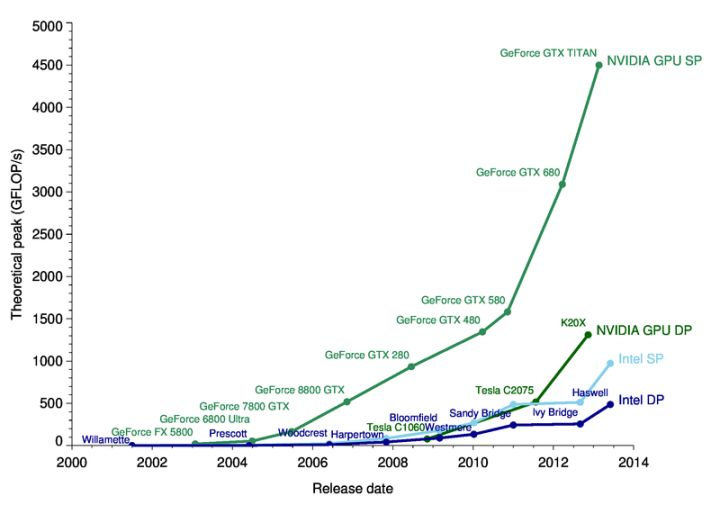
\includegraphics[scale=0.5]{./figures/curve.jpg}
            \caption{\textup{\heiti CPU和GPU单双精度浮点计算能力发展} }
            \label{fig:curve}
        \end{figure}

    \section{实验过程}
        \subsection{问题描述}
        本问题研究的是简单的圆柱绕流问题,物理示意图如图\ref{fig:model}所示。
        \begin{figure}[H]
            \centering
            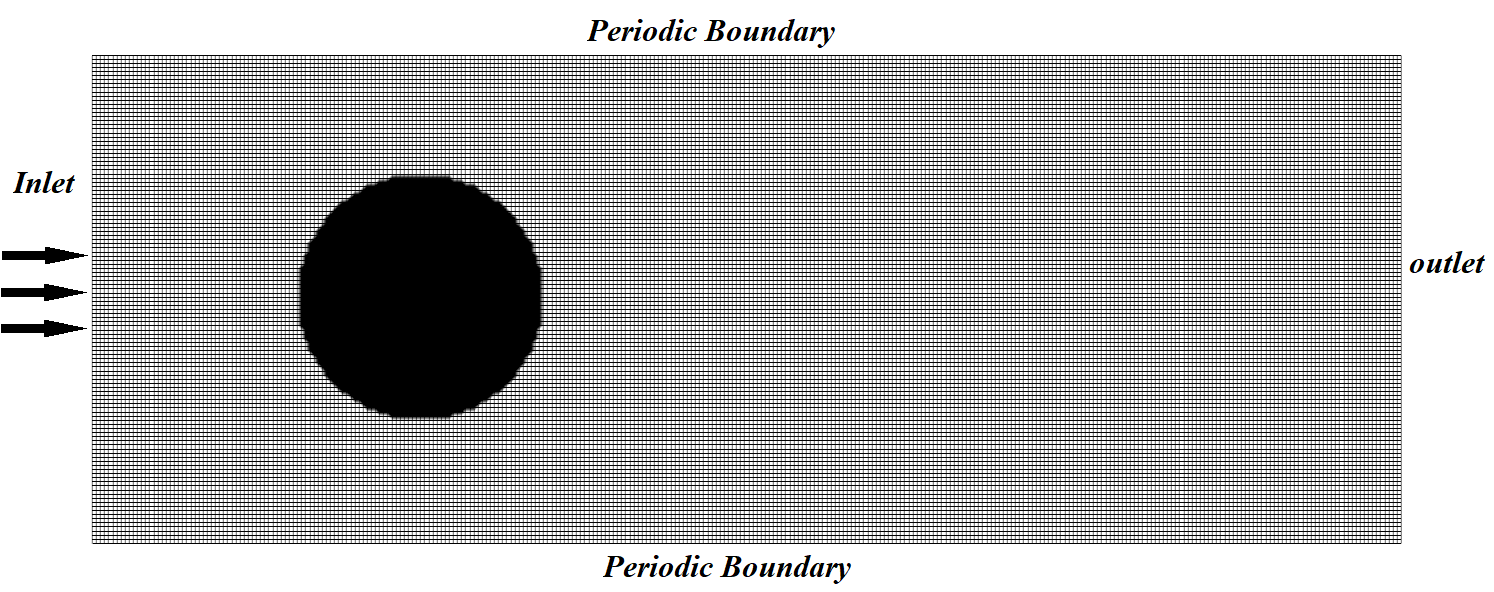
\includegraphics[scale=0.4]{./figures/model.png}
            \caption{\textup{\heiti 计算流场物理示意图} }
            \label{fig:model}
        \end{figure}

        其中计算域的网格$N_x \times N_y$划分为420×160,圆柱的直径为80个网格,圆心的x坐标位于$0.25N_x$处,y坐标位于$0.5N_y$处。
        对于宏观量,我们给定进口来流速度$vxin=0.04$,密度为$roout=1.0$,LBM松弛时间$\tau=0.51$,这是与流体粘性有关的参数。

        对于边界条件,上下边界条件我们采用周期边界条件,左侧进口边界条件根据给定的入口速度$vxin$设置为Zou-He边界条件,
        右侧出口边界条件采用简单的外推边界条件,圆柱的固壁边界使用bounceback边界条件,具体实现代码在函数\texttt{apply\_BCs()}中。

        \subsection{实验设备}
        本文实验平台:操作系统为Microsoft Windows 10。CPU为Intel(R) Core(TM) i5-10500 CPU,主频为3.10 GHz,
        六核心十二线程。显卡为NVIDIA GeForce 1050Ti,显存为4GB,显卡的核心频率为1291-1392MHz,
        部分参数和GPU-Z识别结果如图\ref{fig:GPUZ}和\ref{fig:device}所示。
        
        \begin{figure}[H]
            \centering
            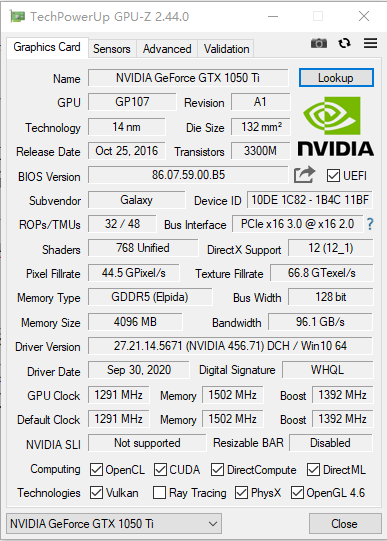
\includegraphics[scale=0.65]{./figures/CUDA-z.png}
            \caption{\textup{\heiti GPU-Z设备识别结果} }
            \label{fig:GPUZ}
        \end{figure}
        \begin{figure}[H]
            \centering
            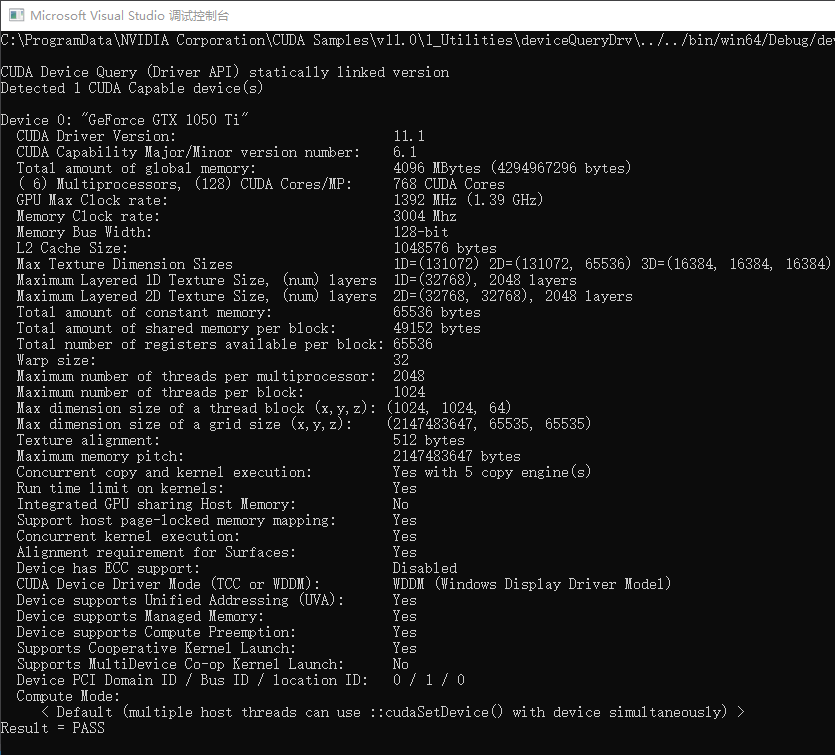
\includegraphics[scale=0.7]{./figures/device.png}
            \caption{\textup{\heiti deviceQuery运行结果} }
            \label{fig:device}
        \end{figure}

        \subsection{数据结构设计}
        对于C语言的串行和OpenMP并行程序,我们分配长度为$N_x\times N_y$的十八个一维float型数组,用于存储九个分布函数f0,f1, $\ldots$,f8
        和临时存储的中间数组tmpf0,tmpf1, $\ldots$,tmpf8。同时,我们还需要同样长度的两个一维float数组u,v和一个一维int数组solid,
        分别用来存储网格点上的两个速度分量以及圆柱固体点的判别标识(其中0代表固体点,1代表流体点)。

        对于CUDA程序,我们在CPU端上同样先分配九个一维float型数组f0,f1, $\ldots$,f8,两个一维float数组u,v和一个一维int数组solid;
        在GPU端上使用\texttt{cudaMallocPitch()}函数分配对应大小的线性数组f0\_data,f1\_data,$\ldots$,f8\_data,和u\_data,v\_data,solid\_data。
        \texttt{cudaMallocPitch()}在分配内存时,为保证数组的每一行的第一个元素的开始地址对齐,每行会多分配一些字节,以保证每行的字节是256的倍数(对齐),
        这样可以提高读取效率,示意图如图\ref{fig:grid}所示。
        \begin{figure}[htbp]
            \centering
            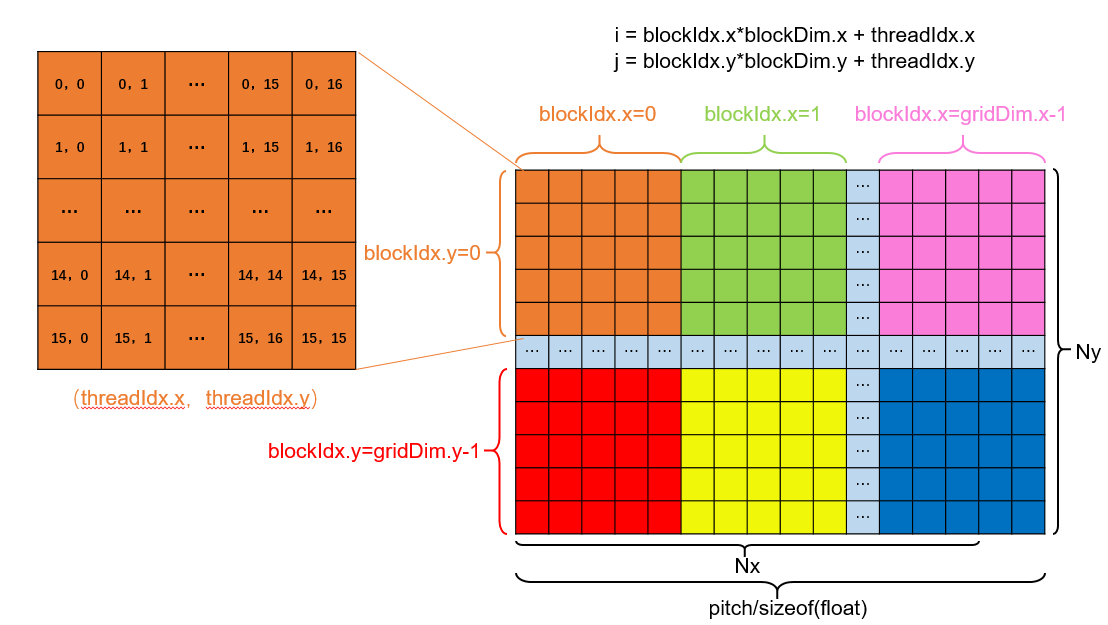
\includegraphics[scale=0.4]{./figures/grid.png}
            \caption{\textup{\heiti 流场网格与数组对应逻辑计算结构} }
            \label{fig:grid}
        \end{figure}

        因为0方向分布函数f0并不会实际参与对流步,所以我们使用\texttt{cudaMallocArray()}仅分配八个CUDA数组f1\_array,f2\_array,$\ldots$,f8\_array。
        从LBM算法特性可以看出,对流过程每个线程读取位置与邻近线程读取位置非常接近,存在大量的空间局部性,纹理内存非常适用于该算法。
        我们预先声明八个的texture<float, 2>类型的2D纹理变量f1\_tex,f2\_tex,$\ldots$,f8\_tex,并使用\texttt{cudaBindTextureToArray()}将CUDA数组与纹理内存绑定起来。

        需要注意的是,因为纹理内存作为一种只读内存,无法通过写操作更新,在对流步前后需要不断通过\texttt{cudaBindTextureToArray()}
        和\texttt{cudaUnbindTexture()}进行绑定和解绑操作。
        从而实现整个流程网格点上分布函数的更新迭代。在核函数\texttt{stream\_kernel()}中,我们使用\texttt{tex2D()}来拾取某个网格点周围点的纹理内存,从而实现对流操作。

        \newpage
        \subsection{流程计算框图}
        具体的流程计算框图如下:
        \begin{figure}[H]
            \centering
            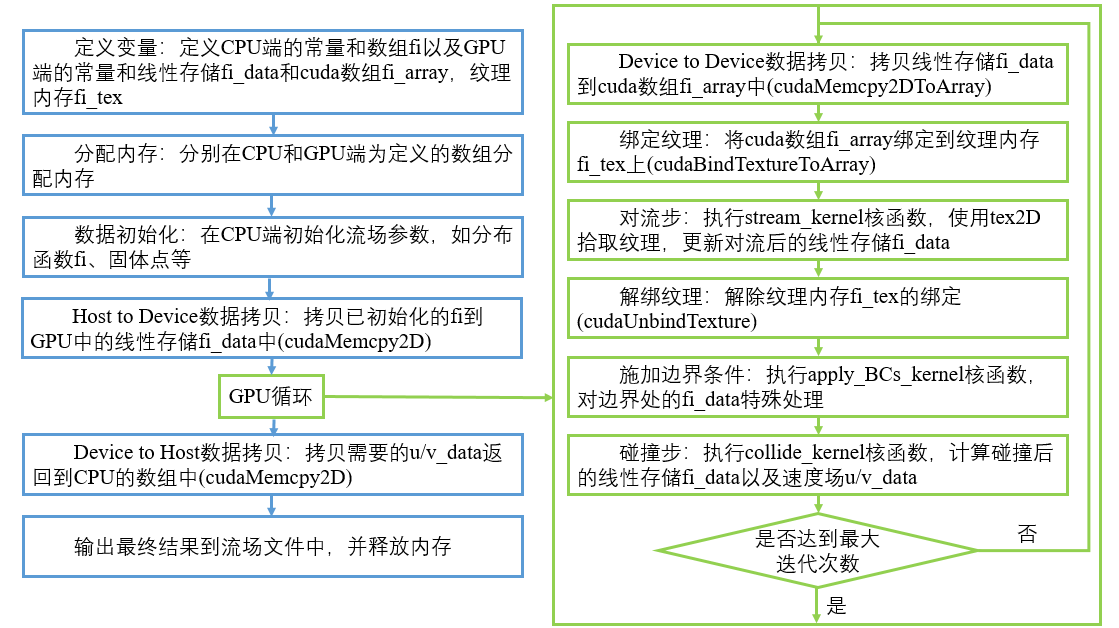
\includegraphics[scale=0.4]{./figures/stream.png}
            \caption{\textup{\heiti 流程计算框图} }
            \label{fig:stream}
        \end{figure}

        \section{结论与分析}
        \subsection{流场结果对比}
        为了验证程序的正确性,我们分别将\texttt{LBM\_C.c},\texttt{LBM\_OpenMP.c}和\texttt{LBM\_CUDA.c}三个程序运行10000步后的每个网格点的速度分量u,v输出到文件\texttt{10000.plt}中,
        并使用后处理软件tecplot绘制涡量云图进行对比,涡量计算公式为$vort=\partial v/\partial x-\partial u/\partial y$,可同时验证速度场u和v的正确性。
        如图\ref{fig:result}所示,三种程序计算结果完全一致,说明三者程序计算正确。

        \begin{figure}[H]
            \centering
            \subfloat[串行]{\includegraphics[width=5.3 in]{./figures/c.png}}\\
            \subfloat[OpenMP并行(四核)]{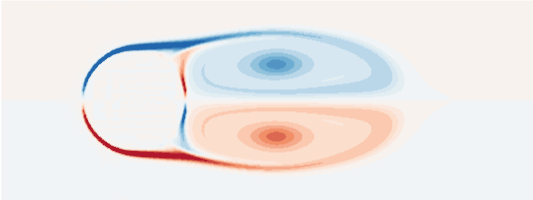
\includegraphics[width=5.3 in]{./figures/openmp.png}}\\
            \subfloat[GPU并行(block:$16\times16$)]{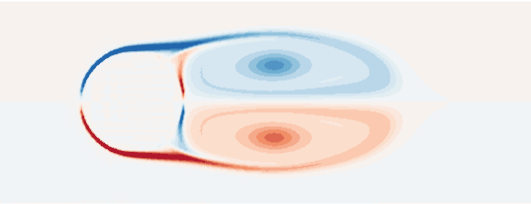
\includegraphics[width=5.3 in]{./figures/cuda.png}}
            \caption{\textup{\heiti 三种程序计算圆柱绕流的涡量云图} }
            \label{fig:result}
        \end{figure}

        \subsection{运行时间对比}
        如表\ref{time}所示是我们程序运行时间的结果。这里我们使用两种计时方法:对于串行和OpenMP并行程序,我们采用的是CPU时钟,
        通过\texttt{clock()}调用并且计算。对于GPU程序,因为核函数与CPU程序是异步执行的,容易带来各种延迟。相比之下,
        继续采用CPU主机端计时就会不够精确(CPU计时仅精确到小数点后三位,GPU时间计时精确到小数点后六位),
        因而我们选择采用CUDA 事件计时API计算时间,并且能确定GPU不同操作的耗时。

        为了减小实验中的随机误差,我们尽量关闭其他后台程序,保证在相同的设备环境下多次运行程序,
        求出最终消耗时间的平均值以及相对于串行程序的加速比。理想情况下,使用OpenMP四核并行最后的加速比应该能达到4.0,
        但实际操作过程存在任务切换以及调度等时间开销,最终的加速比也只有3.4左右。对于CUDA并行,
        可以发现GPU加速比能够达到将近20,远远优于OpenMP的加速效果。考虑到实验所使用的CPU和GPU价格相近,
        CPU想达到相同的加速效果需要的成本大得多,这也是近年来超级计算机越来越多使用GPU进行加速计算的原因。

        \begin{table}[htp]
            \centering %表格居中放置 
            \caption{\textup{\heiti 各程序计算时间对比}}\label{time} %用于引用
            \begin{tabular}{|c|c|c|c|}
            \hline
                & CPU串行  & OpenMP四核 & \begin{tabular}[c]{@{}c@{}}CUDA\\ (block:16×16)\end{tabular} \\ \hline
            1   & 39.960 & 11.376   & 2.172047                                                   \\
            2   & 39.934 & 11.680   & 2.183745                                                   \\
            3   & 39.998 & 11.407   & 2.174925                                                   \\
            4   & 39.984 & 12.162   & 2.167604                                                   \\
            5   & 39.935 & 11.897   & 2.182287                                                   \\
            6   & 39.939 & 11.712   & 2.170362                                                   \\
            7   & 39.925 & 11.818   & 2.188568                                                   \\
            8   & 39.928 & 12.055   & 2.175561                                                   \\ \hline
            均值  & 39.950 & 11.763   & 2.176887                                                   \\ \hline
            加速比 & 1.000  & 3.396    & 18.35206                                                   \\ \hline
            \end{tabular}
        \end{table}

        \subsection{参数影响}
        \subsubsection{CPU并行核数}
        众所周知,加速比是衡量一个并行算法是否有效的重要指标,但实际应用中往往还要综合考虑并行效率来选择合适的硬件环境。
        并行效率,即用加速比除以并行核数,值越高的程序表明越充分发挥了处理器的作用。

        为了研究CPU核数对并行效率的影响,我们通过\texttt{omp\_set\_num\_threads()}函数改变并行核数,
        分别研究了1/2/4/6核下的并行计算效率,相关结果在表\ref{timecpu}和图\ref{fig:1}中。如图所示,随着核数增加,加速比也逐渐增加,
        但并不是呈线性相关性。在六核时加速比只有3.822,相比四核提升不大。除了程序中存在串行部分外,
        还因为即使计算机关闭大部分应用程序,依然有一些系统程序占用CPU运行,所以并不能完全发挥六核并行的效果。

        \begin{table}[]
            \centering %表格居中放置 
            \caption{\textup{\heiti 不同CPU核数并行程序计算时间对比}}\label{timecpu} %用于引用
            \begin{tabular}{|c|c|c|c|c|}
            \hline
                 & 单核     & 双核      & 四核       & 六核       \\ \hline
            1    & 39.960 & 21.372  & 11.376   & 10.398   \\
            2    & 39.934 & 21.473  & 11.680   & 10.593   \\
            3    & 39.998 & 21.410  & 11.407   & 10.225   \\
            4    & 39.984 & 21.259  & 12.162   & 10.655   \\
            5    & 39.935 & 21.223  & 11.897   & 10.582   \\
            6    & 39.939 & 21.335  & 11.712   & 10.494   \\
            7    & 39.925 & 21.219  & 11.818   & 9.964    \\
            8    & 39.928 & 21.295  & 12.055   & 10.717   \\ \hline
            均值   & 39.950 & 21.323  & 11.763   & 10.454   \\ \hline
            加速比  & 1.000  & 1.874   & 3.396    & 3.822    \\ \hline
            并行效率 & 1.000  & 0.93678 & 0.849042 & 0.636954 \\ \hline
            \end{tabular}
        \end{table}

        \begin{figure}[H]
            \centering
            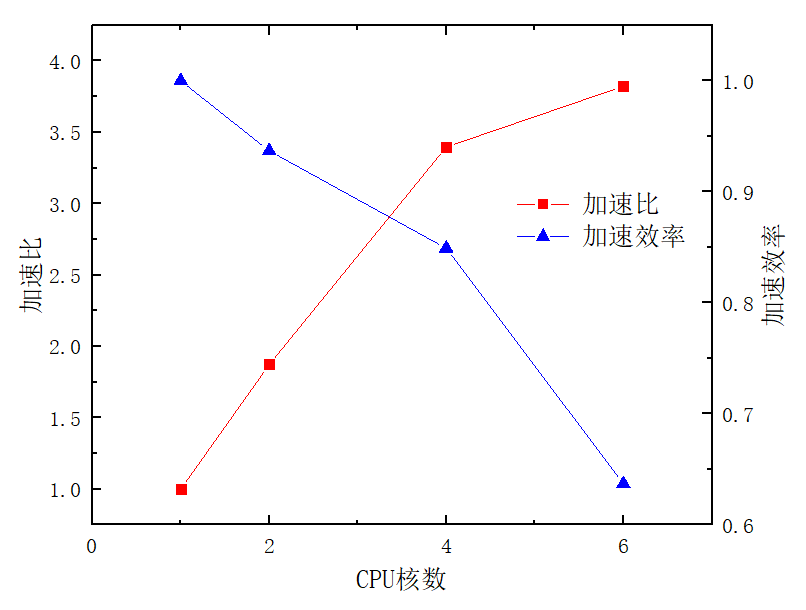
\includegraphics[scale=0.40]{./figures/fig1.png}
            \caption{\textup{\heiti 不同CPU核数并行程序加速比和并行效率对比} }
            \label{fig:1}
        \end{figure}
        
        \subsubsection{GPU线程块大小}
        在 CUDA 架构下,执行时的最小单位是thread,若干个 thread 可以组成一个block,每一个 block 所能包含的 thread 数目是有限的
        (最多1024个),执行相同程序的 block又可以组成grid。

        但从线程运行的原理来看,block中的线程数量并不是全部使用完最好,相反在达到一定大小后,一味地增加线程也不会取得性能的提升,
        反而有可能会让性能下降。线程数达到隐藏各种延迟的程度后,之后线程数量的提升就并无太大的作用。
        所以,存在一个最优的block大小,使得加速效果最好。

        这里,我们分别实验了block大小为$8\times8$,$16\times16$,$16\times32$,$32\times16$,$32\times32$五种情况,
        并将计算结果统计在表\ref{timegpu}和图\ref{fig:2}中。从图中可见,线程块的大小过大或者过小都会让加速效果下降,最优的线程块配置在$16\times16$附近。

        \begin{table}[]
            \centering %表格居中放置 
            \caption{\textup{\heiti 不同GPU线程块大小并行程序计算时间对比}}\label{timegpu} %用于引用
            \begin{tabular}{|c|c|c|c|c|c|}
            \hline
            线程块大小 & 8×8       & 16×16     & 16×32     & 32×16     & 32×32     \\ \hline
            1     & 2.260829  & 2.172047  & 2.188429  & 2.219378  & 2.238027  \\
            2     & 2.255240  & 2.183745  & 2.190795  & 2.217793  & 2.233487  \\
            3     & 2.254273  & 2.174925  & 2.189309  & 2.217046  & 2.235491  \\
            4     & 2.258347  & 2.167604  & 2.186552  & 2.229166  & 2.245697  \\
            5     & 2.258553  & 2.182287  & 2.198995  & 2.217546  & 2.236075  \\
            6     & 2.275972  & 2.170362  & 2.190464  & 2.218092  & 2.242517  \\
            7     & 2.278869  & 2.188568  & 2.195127  & 2.221389  & 2.244022  \\
            8     & 2.275238  & 2.175561  & 2.185740  & 2.216016  & 2.234186  \\ \hline
            均值    & 2.264665  & 2.176887  & 2.190676  & 2.219553  & 2.238688  \\ \hline
            加速比   & 17.640743 & 18.352063 & 18.236558 & 17.999297 & 17.845443 \\ \hline
            \end{tabular}
        \end{table}

        \begin{figure}[H]
            \centering
            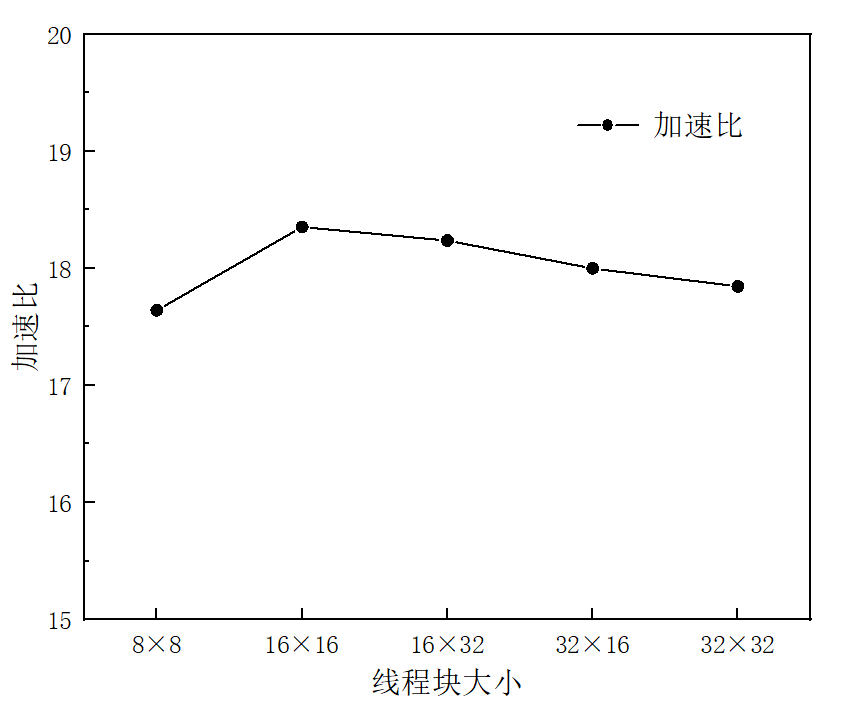
\includegraphics[scale=0.38]{./figures/fig2.png}
            \caption{\textup{\heiti 不同GPU线程块大小并行程序加速比对比} }
            \label{fig:2}
        \end{figure}
        
        \section{心得体会}
        通过完成本次GPU并行计算的大作业,我回顾了所学的有关C语言的相关理论,同时也再次加深对LBM算法实现的理解。

        首先是对这次实验的一些经验性的总结:(1)对于CUDA的安装,一定要选择适配自己的显卡版本,且对于这种底层的语言安装最好安装在C盘,
        否则在设置环境变量以及调用库函数时,经常会找不到路径;(2)程序对比实验时,一定要保证属性设置完全一致, 
        Release版本的程序相比Debug版本也有很大的速度优化,除此以外O1/O2/O3优化也会对程序速度产生很大影响。
        (3)对于线程块的大小,并不是越大越好,存在最优的配置,需要靠自行实验得出。

        作为计算流体力学专业的学生,事实上本课题组使用的很多Fortran代码都使用了并行计算的方法,包括MPI或者OpenMP并行。
        CUDA作为一种新兴的并行架构,对于加速流体力学计算有很广泛的前景。这次模拟的问题只是流体力学中很简单的问题,
        实际问题计算中往往还涉及到复杂的流固耦合问题等等,这对于如何使用CUDA实现还需要重新设计程序结构。

        最后,要感谢老师上课的讲解,虽然之前一直在使用课题组相关并行代码,但对并行计算的内容了解甚少。
        同时也要感谢同学的建议,在代码debug的方法对我的启发很大,才能顺利完成本次大作业。



\end{document}